% Options for packages loaded elsewhere
\PassOptionsToPackage{unicode}{hyperref}
\PassOptionsToPackage{hyphens}{url}
\PassOptionsToPackage{dvipsnames,svgnames,x11names}{xcolor}
%
\documentclass[
  letterpaper,
  DIV=11,
  numbers=noendperiod]{scrartcl}

\usepackage{amsmath,amssymb}
\usepackage{iftex}
\ifPDFTeX
  \usepackage[T1]{fontenc}
  \usepackage[utf8]{inputenc}
  \usepackage{textcomp} % provide euro and other symbols
\else % if luatex or xetex
  \usepackage{unicode-math}
  \defaultfontfeatures{Scale=MatchLowercase}
  \defaultfontfeatures[\rmfamily]{Ligatures=TeX,Scale=1}
\fi
\usepackage{lmodern}
\ifPDFTeX\else  
    % xetex/luatex font selection
\fi
% Use upquote if available, for straight quotes in verbatim environments
\IfFileExists{upquote.sty}{\usepackage{upquote}}{}
\IfFileExists{microtype.sty}{% use microtype if available
  \usepackage[]{microtype}
  \UseMicrotypeSet[protrusion]{basicmath} % disable protrusion for tt fonts
}{}
\makeatletter
\@ifundefined{KOMAClassName}{% if non-KOMA class
  \IfFileExists{parskip.sty}{%
    \usepackage{parskip}
  }{% else
    \setlength{\parindent}{0pt}
    \setlength{\parskip}{6pt plus 2pt minus 1pt}}
}{% if KOMA class
  \KOMAoptions{parskip=half}}
\makeatother
\usepackage{xcolor}
\setlength{\emergencystretch}{3em} % prevent overfull lines
\setcounter{secnumdepth}{-\maxdimen} % remove section numbering
% Make \paragraph and \subparagraph free-standing
\ifx\paragraph\undefined\else
  \let\oldparagraph\paragraph
  \renewcommand{\paragraph}[1]{\oldparagraph{#1}\mbox{}}
\fi
\ifx\subparagraph\undefined\else
  \let\oldsubparagraph\subparagraph
  \renewcommand{\subparagraph}[1]{\oldsubparagraph{#1}\mbox{}}
\fi

\usepackage{color}
\usepackage{fancyvrb}
\newcommand{\VerbBar}{|}
\newcommand{\VERB}{\Verb[commandchars=\\\{\}]}
\DefineVerbatimEnvironment{Highlighting}{Verbatim}{commandchars=\\\{\}}
% Add ',fontsize=\small' for more characters per line
\usepackage{framed}
\definecolor{shadecolor}{RGB}{241,243,245}
\newenvironment{Shaded}{\begin{snugshade}}{\end{snugshade}}
\newcommand{\AlertTok}[1]{\textcolor[rgb]{0.68,0.00,0.00}{#1}}
\newcommand{\AnnotationTok}[1]{\textcolor[rgb]{0.37,0.37,0.37}{#1}}
\newcommand{\AttributeTok}[1]{\textcolor[rgb]{0.40,0.45,0.13}{#1}}
\newcommand{\BaseNTok}[1]{\textcolor[rgb]{0.68,0.00,0.00}{#1}}
\newcommand{\BuiltInTok}[1]{\textcolor[rgb]{0.00,0.23,0.31}{#1}}
\newcommand{\CharTok}[1]{\textcolor[rgb]{0.13,0.47,0.30}{#1}}
\newcommand{\CommentTok}[1]{\textcolor[rgb]{0.37,0.37,0.37}{#1}}
\newcommand{\CommentVarTok}[1]{\textcolor[rgb]{0.37,0.37,0.37}{\textit{#1}}}
\newcommand{\ConstantTok}[1]{\textcolor[rgb]{0.56,0.35,0.01}{#1}}
\newcommand{\ControlFlowTok}[1]{\textcolor[rgb]{0.00,0.23,0.31}{#1}}
\newcommand{\DataTypeTok}[1]{\textcolor[rgb]{0.68,0.00,0.00}{#1}}
\newcommand{\DecValTok}[1]{\textcolor[rgb]{0.68,0.00,0.00}{#1}}
\newcommand{\DocumentationTok}[1]{\textcolor[rgb]{0.37,0.37,0.37}{\textit{#1}}}
\newcommand{\ErrorTok}[1]{\textcolor[rgb]{0.68,0.00,0.00}{#1}}
\newcommand{\ExtensionTok}[1]{\textcolor[rgb]{0.00,0.23,0.31}{#1}}
\newcommand{\FloatTok}[1]{\textcolor[rgb]{0.68,0.00,0.00}{#1}}
\newcommand{\FunctionTok}[1]{\textcolor[rgb]{0.28,0.35,0.67}{#1}}
\newcommand{\ImportTok}[1]{\textcolor[rgb]{0.00,0.46,0.62}{#1}}
\newcommand{\InformationTok}[1]{\textcolor[rgb]{0.37,0.37,0.37}{#1}}
\newcommand{\KeywordTok}[1]{\textcolor[rgb]{0.00,0.23,0.31}{#1}}
\newcommand{\NormalTok}[1]{\textcolor[rgb]{0.00,0.23,0.31}{#1}}
\newcommand{\OperatorTok}[1]{\textcolor[rgb]{0.37,0.37,0.37}{#1}}
\newcommand{\OtherTok}[1]{\textcolor[rgb]{0.00,0.23,0.31}{#1}}
\newcommand{\PreprocessorTok}[1]{\textcolor[rgb]{0.68,0.00,0.00}{#1}}
\newcommand{\RegionMarkerTok}[1]{\textcolor[rgb]{0.00,0.23,0.31}{#1}}
\newcommand{\SpecialCharTok}[1]{\textcolor[rgb]{0.37,0.37,0.37}{#1}}
\newcommand{\SpecialStringTok}[1]{\textcolor[rgb]{0.13,0.47,0.30}{#1}}
\newcommand{\StringTok}[1]{\textcolor[rgb]{0.13,0.47,0.30}{#1}}
\newcommand{\VariableTok}[1]{\textcolor[rgb]{0.07,0.07,0.07}{#1}}
\newcommand{\VerbatimStringTok}[1]{\textcolor[rgb]{0.13,0.47,0.30}{#1}}
\newcommand{\WarningTok}[1]{\textcolor[rgb]{0.37,0.37,0.37}{\textit{#1}}}

\providecommand{\tightlist}{%
  \setlength{\itemsep}{0pt}\setlength{\parskip}{0pt}}\usepackage{longtable,booktabs,array}
\usepackage{calc} % for calculating minipage widths
% Correct order of tables after \paragraph or \subparagraph
\usepackage{etoolbox}
\makeatletter
\patchcmd\longtable{\par}{\if@noskipsec\mbox{}\fi\par}{}{}
\makeatother
% Allow footnotes in longtable head/foot
\IfFileExists{footnotehyper.sty}{\usepackage{footnotehyper}}{\usepackage{footnote}}
\makesavenoteenv{longtable}
\usepackage{graphicx}
\makeatletter
\def\maxwidth{\ifdim\Gin@nat@width>\linewidth\linewidth\else\Gin@nat@width\fi}
\def\maxheight{\ifdim\Gin@nat@height>\textheight\textheight\else\Gin@nat@height\fi}
\makeatother
% Scale images if necessary, so that they will not overflow the page
% margins by default, and it is still possible to overwrite the defaults
% using explicit options in \includegraphics[width, height, ...]{}
\setkeys{Gin}{width=\maxwidth,height=\maxheight,keepaspectratio}
% Set default figure placement to htbp
\makeatletter
\def\fps@figure{htbp}
\makeatother

\usepackage{float}
\usepackage{tabularray}
\usepackage[normalem]{ulem}
\usepackage{graphicx}
\UseTblrLibrary{booktabs}
\UseTblrLibrary{siunitx}
\NewTableCommand{\tinytableDefineColor}[3]{\definecolor{#1}{#2}{#3}}
\newcommand{\tinytableTabularrayUnderline}[1]{\underline{#1}}
\newcommand{\tinytableTabularrayStrikeout}[1]{\sout{#1}}
\KOMAoption{captions}{tableheading}
\makeatletter
\@ifpackageloaded{caption}{}{\usepackage{caption}}
\AtBeginDocument{%
\ifdefined\contentsname
  \renewcommand*\contentsname{Table of contents}
\else
  \newcommand\contentsname{Table of contents}
\fi
\ifdefined\listfigurename
  \renewcommand*\listfigurename{List of Figures}
\else
  \newcommand\listfigurename{List of Figures}
\fi
\ifdefined\listtablename
  \renewcommand*\listtablename{List of Tables}
\else
  \newcommand\listtablename{List of Tables}
\fi
\ifdefined\figurename
  \renewcommand*\figurename{Figure}
\else
  \newcommand\figurename{Figure}
\fi
\ifdefined\tablename
  \renewcommand*\tablename{Table}
\else
  \newcommand\tablename{Table}
\fi
}
\@ifpackageloaded{float}{}{\usepackage{float}}
\floatstyle{ruled}
\@ifundefined{c@chapter}{\newfloat{codelisting}{h}{lop}}{\newfloat{codelisting}{h}{lop}[chapter]}
\floatname{codelisting}{Listing}
\newcommand*\listoflistings{\listof{codelisting}{List of Listings}}
\makeatother
\makeatletter
\makeatother
\makeatletter
\@ifpackageloaded{caption}{}{\usepackage{caption}}
\@ifpackageloaded{subcaption}{}{\usepackage{subcaption}}
\makeatother
\ifLuaTeX
  \usepackage{selnolig}  % disable illegal ligatures
\fi
\usepackage{bookmark}

\IfFileExists{xurl.sty}{\usepackage{xurl}}{} % add URL line breaks if available
\urlstyle{same} % disable monospaced font for URLs
\hypersetup{
  pdftitle={Homework 3},
  pdfauthor={Rebecca-Jane Gullette},
  colorlinks=true,
  linkcolor={blue},
  filecolor={Maroon},
  citecolor={Blue},
  urlcolor={Blue},
  pdfcreator={LaTeX via pandoc}}

\title{Homework 3}
\author{Rebecca-Jane Gullette}
\date{2024-06-08}

\begin{document}
\maketitle

\renewcommand*\contentsname{Table of contents}
{
\hypersetup{linkcolor=}
\setcounter{tocdepth}{3}
\tableofcontents
}
https://github.com/rebecca-jane-gullette/Gullette-RebeccaJane\_homework-03.git

\subsection{Read in Packages and Data}\label{read-in-packages-and-data}

\begin{Shaded}
\begin{Highlighting}[]
\FunctionTok{library}\NormalTok{(tidyverse) }\CommentTok{\# clean data}
\FunctionTok{library}\NormalTok{(readxl) }\CommentTok{\# read in excel file }
\FunctionTok{library}\NormalTok{(here) }\CommentTok{\# find file}
\FunctionTok{library}\NormalTok{(janitor) }\CommentTok{\# clean data}
\FunctionTok{library}\NormalTok{(GGally) }\CommentTok{\# data visualization }
\FunctionTok{library}\NormalTok{(MuMIn) }\CommentTok{\# model selection}
\FunctionTok{library}\NormalTok{(ggeffects) }\CommentTok{\# model predictions}
\FunctionTok{library}\NormalTok{(gtsummary) }\CommentTok{\# summary tables}
\FunctionTok{library}\NormalTok{(flextable) }\CommentTok{\# flex tables}
\FunctionTok{library}\NormalTok{(modelsummary) }\CommentTok{\# model tables}
\FunctionTok{library}\NormalTok{(tinytex) }\CommentTok{\# render to pdf }

\NormalTok{drought\_exp }\OtherTok{\textless{}{-}} \FunctionTok{read\_xlsx}\NormalTok{(}\AttributeTok{path =} \FunctionTok{here}\NormalTok{(}\StringTok{"data"}\NormalTok{, }\CommentTok{\# reading in data}
                                     \StringTok{"Valliere\_etal\_EcoApps\_Data.xlsx"}\NormalTok{),}
                         \AttributeTok{sheet =} \StringTok{"First Harvest"}\NormalTok{)}
\end{Highlighting}
\end{Shaded}

\section{Problem 1}\label{problem-1}

\subsection{a. code and annotations}\label{a.-code-and-annotations}

\begin{Shaded}
\begin{Highlighting}[]
\NormalTok{drought\_exp\_clean }\OtherTok{\textless{}{-}}\NormalTok{ drought\_exp }\SpecialCharTok{\%\textgreater{}\%} \CommentTok{\# cleaning data}
  \FunctionTok{clean\_names}\NormalTok{() }\SpecialCharTok{\%\textgreater{}\%} \CommentTok{\# changing column names}
  \FunctionTok{mutate}\NormalTok{(}\AttributeTok{species\_name =} \FunctionTok{case\_when}\NormalTok{( }\CommentTok{\# adding column for species scientific names}
\NormalTok{    species }\SpecialCharTok{==} \StringTok{"ENCCAL"} \SpecialCharTok{\textasciitilde{}} \StringTok{"Encelia californica"}\NormalTok{, }\CommentTok{\# bush sunflower}
\NormalTok{    species }\SpecialCharTok{==} \StringTok{"ESCCAL"} \SpecialCharTok{\textasciitilde{}} \StringTok{"Eschscholzia californica"}\NormalTok{, }\CommentTok{\# California poppy}
\NormalTok{    species }\SpecialCharTok{==} \StringTok{"PENCEN"} \SpecialCharTok{\textasciitilde{}} \StringTok{"Penstemon centranthifolius"}\NormalTok{, }\CommentTok{\# Scarlet bugler}
\NormalTok{    species }\SpecialCharTok{==} \StringTok{"GRICAM"} \SpecialCharTok{\textasciitilde{}} \StringTok{"Grindelia camporum"}\NormalTok{, }\CommentTok{\# great valley gumweed}
\NormalTok{    species }\SpecialCharTok{==} \StringTok{"SALLEU"} \SpecialCharTok{\textasciitilde{}} \StringTok{"Salvia leucophylla"}\NormalTok{, }\CommentTok{\# Purple sage}
\NormalTok{    species }\SpecialCharTok{==} \StringTok{"STIPUL"} \SpecialCharTok{\textasciitilde{}} \StringTok{"Nasella pulchra"}\NormalTok{, }\CommentTok{\# Purple needlegrass}
\NormalTok{    species }\SpecialCharTok{==} \StringTok{"LOTSCO"} \SpecialCharTok{\textasciitilde{}} \StringTok{"Acmispon glaber"} \CommentTok{\# deerweed}
\NormalTok{  )) }\SpecialCharTok{\%\textgreater{}\%} 
  \FunctionTok{relocate}\NormalTok{(species\_name, }\AttributeTok{.after =}\NormalTok{ species) }\SpecialCharTok{\%\textgreater{}\%} \CommentTok{\# move species\_name column after species}
  \FunctionTok{mutate}\NormalTok{(}\AttributeTok{water\_treatment =} \FunctionTok{case\_when}\NormalTok{( }\CommentTok{\# adding column with full treatment names}
\NormalTok{    water }\SpecialCharTok{==} \StringTok{"WW"} \SpecialCharTok{\textasciitilde{}} \StringTok{"Well watered"}\NormalTok{,}
\NormalTok{    water }\SpecialCharTok{==} \StringTok{"DS"} \SpecialCharTok{\textasciitilde{}} \StringTok{"Drought stressed"}
\NormalTok{  )) }\SpecialCharTok{\%\textgreater{}\%} 
  \FunctionTok{relocate}\NormalTok{(water\_treatment, }\AttributeTok{.after =}\NormalTok{ water) }\CommentTok{\# moving water\_treatment column after water}

\CommentTok{\# models from workshop }
\NormalTok{model0 }\OtherTok{\textless{}{-}} \FunctionTok{lm}\NormalTok{(total\_g }\SpecialCharTok{\textasciitilde{}} \DecValTok{1}\NormalTok{, }\CommentTok{\# formula null model}
             \AttributeTok{data =}\NormalTok{ drought\_exp\_clean) }\CommentTok{\# data frame}

\NormalTok{model1 }\OtherTok{\textless{}{-}} \FunctionTok{lm}\NormalTok{(total\_g }\SpecialCharTok{\textasciitilde{}}\NormalTok{ sla }\SpecialCharTok{+}\NormalTok{ water\_treatment }\SpecialCharTok{+}\NormalTok{ species\_name, }\CommentTok{\# saturated model}
             \AttributeTok{data =}\NormalTok{ drought\_exp\_clean) }

\NormalTok{model2 }\OtherTok{\textless{}{-}} \FunctionTok{lm}\NormalTok{(total\_g }\SpecialCharTok{\textasciitilde{}}\NormalTok{ sla }\SpecialCharTok{+}\NormalTok{ water\_treatment, }\CommentTok{\# total biomass as a function of SLA and water treatment}
             \AttributeTok{data =}\NormalTok{ drought\_exp\_clean)}

\NormalTok{model3 }\OtherTok{\textless{}{-}} \FunctionTok{lm}\NormalTok{(total\_g }\SpecialCharTok{\textasciitilde{}}\NormalTok{ sla }\SpecialCharTok{+}\NormalTok{ species\_name, }\CommentTok{\# total biomass as a function of SLA and species }
             \AttributeTok{data =}\NormalTok{ drought\_exp\_clean)}

\CommentTok{\# additional model}
\NormalTok{model4 }\OtherTok{\textless{}{-}} \FunctionTok{lm}\NormalTok{(total\_g }\SpecialCharTok{\textasciitilde{}}\NormalTok{ water\_treatment }\SpecialCharTok{+}\NormalTok{ species\_name, }\CommentTok{\# total biomass as a function of water treatment and species}
             \AttributeTok{data =}\NormalTok{ drought\_exp\_clean)}



\NormalTok{ model\_table }\OtherTok{\textless{}{-}}\NormalTok{ modelsummary}\SpecialCharTok{::}\FunctionTok{modelsummary}\NormalTok{( }\CommentTok{\# create a table summarizing the models}
  \FunctionTok{list}\NormalTok{( }\CommentTok{\# selecting the models to include}
    \StringTok{"Null Model: No Predictors"} \OtherTok{=}\NormalTok{ model0, }\CommentTok{\# changing model names to indicate predictors }
    \StringTok{"Model 1: All Predictors"} \OtherTok{=}\NormalTok{ model1,}
    \StringTok{"Model 2: SLA and Water Treatment"} \OtherTok{=}\NormalTok{ model2,}
    \StringTok{"Model 3: SLA and Species"} \OtherTok{=}\NormalTok{ model3,}
    \StringTok{"Model 4: Water Treatment and Species"} \OtherTok{=}\NormalTok{ model4}
\NormalTok{  ))}
\end{Highlighting}
\end{Shaded}

Table 1. Comparison of Five Models of Total Biomass and Three
Predictors: Specific Leaf Area, Water Treatment, and Species.

\begin{Shaded}
\begin{Highlighting}[]
\NormalTok{model\_table }\CommentTok{\# display table of models}
\end{Highlighting}
\end{Shaded}

\begin{table}
\centering
\begin{tblr}[         %% tabularray outer open
]                     %% tabularray outer close
{                     %% tabularray inner open
colspec={Q[]Q[]Q[]Q[]Q[]Q[]},
column{1}={halign=l,},
column{2}={halign=c,},
column{3}={halign=c,},
column{4}={halign=c,},
column{5}={halign=c,},
column{6}={halign=c,},
hline{20}={1,2,3,4,5,6}{solid, 0.05em, black},
}                     %% tabularray inner close
\toprule
& Null Model: No Predictors & Model 1: All Predictors & Model 2: SLA and Water Treatment & Model 3: SLA and Species & Model 4: Water Treatment and Species \\ \midrule %% TinyTableHeader
(Intercept)                              & \num{0.279}   & \num{0.080}   & \num{0.047}   & \num{-0.033}  & \num{0.055}   \\
& (\num{0.017}) & (\num{0.056}) & (\num{0.054}) & (\num{0.067}) & (\num{0.025}) \\
sla                                      &                & \num{0.000}   & \num{0.001}   & \num{0.001}   &                \\
&                & (\num{0.000}) & (\num{0.000}) & (\num{0.001}) &                \\
water\_treatmentWell watered            &                & \num{0.122}   & \num{0.090}   &                & \num{0.117}   \\
&                & (\num{0.020}) & (\num{0.029}) &                & (\num{0.017}) \\
species\_nameEncelia californica        &                & \num{0.238}   &                & \num{0.115}   & \num{0.218}   \\
&                & (\num{0.051}) &                & (\num{0.059}) & (\num{0.032}) \\
species\_nameEschscholzia californica   &                & \num{0.234}   &                & \num{0.222}   & \num{0.232}   \\
&                & (\num{0.033}) &                & (\num{0.041}) & (\num{0.032}) \\
species\_nameGrindelia camporum         &                & \num{0.330}   &                & \num{0.226}   & \num{0.313}   \\
&                & (\num{0.047}) &                & (\num{0.054}) & (\num{0.032}) \\
species\_nameNasella pulchra            &                & \num{0.241}   &                & \num{0.168}   & \num{0.229}   \\
&                & (\num{0.040}) &                & (\num{0.048}) & (\num{0.032}) \\
species\_namePenstemon centranthifolius &                & \num{0.061}   &                & \num{-0.006}  & \num{0.050}   \\
&                & (\num{0.039}) &                & (\num{0.047}) & (\num{0.032}) \\
species\_nameSalvia leucophylla         &                & \num{0.117}   &                & \num{0.139}   & \num{0.120}   \\
&                & (\num{0.033}) &                & (\num{0.041}) & (\num{0.032}) \\
Num.Obs.                                 & \num{70}      & \num{70}      & \num{70}      & \num{70}      & \num{70}      \\
R2                                       & \num{0.000}   & \num{0.755}   & \num{0.303}   & \num{0.610}   & \num{0.754}   \\
R2 Adj.                                  & \num{0.000}   & \num{0.722}   & \num{0.282}   & \num{0.566}   & \num{0.726}   \\
AIC                                      & \num{-75.2}   & \num{-157.5}  & \num{-96.4}   & \num{-127.1}  & \num{-159.2}  \\
BIC                                      & \num{-70.7}   & \num{-135.0}  & \num{-87.4}   & \num{-106.8}  & \num{-139.0}  \\
Log.Lik.                                 & \num{39.580}  & \num{88.741}  & \num{52.220}  & \num{72.538}  & \num{88.598}  \\
RMSE                                     & \num{0.14}    & \num{0.07}    & \num{0.11}    & \num{0.09}    & \num{0.07}    \\
\bottomrule
\end{tblr}
\end{table}

\subsection{b. Write a 5-6 sentence ``statistical methods''
section.}\label{b.-write-a-5-6-sentence-statistical-methods-section.}

To examine the influence of specific leaf area (SLA), water treatment,
and species on the total biomass of plants in California I created 5
linear models with different combinations of predictor variables. The
null model had no predictors, model 1 included all predictors, model 2
looked at SLA and water treatment, model 3 looked at SLA and species,
and model 4 looked at the effect of water treatment and species on total
biomass. To determine the model that best predicts total biomass I used
the model.sel() function from the MuMin package which calculated the
lowest AIC and a delta of 0 for Model 4. Before concluding that this was
the final model I evaluated it for the assumptions of a linear model
using the diagnostic plots and the residuals follow a linear pattern on
the QQ plot and the residuals are homoscedastic and normally
distributed.

\subsection{c.~Make a visualization of the model predictions with
underlying data for your ``best''
model.}\label{c.-make-a-visualization-of-the-model-predictions-with-underlying-data-for-your-best-model.}

\begin{Shaded}
\begin{Highlighting}[]
\NormalTok{model\_preds4 }\OtherTok{\textless{}{-}} \FunctionTok{ggpredict}\NormalTok{(model4, }\CommentTok{\# create data frame with model predictions}
                         \AttributeTok{terms =} \FunctionTok{c}\NormalTok{(}\StringTok{"water\_treatment"}\NormalTok{, }
                                   \StringTok{"species\_name"}\NormalTok{))}

\NormalTok{model\_preds4\_for\_plotting }\OtherTok{\textless{}{-}}\NormalTok{ model\_preds4 }\SpecialCharTok{\%\textgreater{}\%} \CommentTok{\# creating new data frame of model predictions to plot}
  \FunctionTok{rename}\NormalTok{(}\AttributeTok{water\_treatment =}\NormalTok{ x, }\CommentTok{\# renaming columns to be easier to work with}
         \AttributeTok{species\_name =}\NormalTok{ group)}

\FunctionTok{ggplot}\NormalTok{() }\SpecialCharTok{+} \CommentTok{\# creating a plot}
  \FunctionTok{geom\_point}\NormalTok{(}\AttributeTok{data =}\NormalTok{ drought\_exp\_clean, }\CommentTok{\# plotting underlying data }
             \FunctionTok{aes}\NormalTok{(}\AttributeTok{x =}\NormalTok{ water\_treatment,}
                 \AttributeTok{y =}\NormalTok{ total\_g,}
                 \AttributeTok{color =}\NormalTok{ water\_treatment), }\CommentTok{\# creating different colors for water treatment}
             \AttributeTok{position =} \FunctionTok{position\_jitter}\NormalTok{(}\AttributeTok{width =} \FloatTok{0.1}\NormalTok{, }\AttributeTok{height =} \DecValTok{0}\NormalTok{), }\CommentTok{\# jittering points}
             \AttributeTok{size =} \FloatTok{0.8}\NormalTok{,}
             \AttributeTok{alpha =} \FloatTok{0.3}\NormalTok{) }\SpecialCharTok{+} \CommentTok{\# making underlying data transparent}
  \FunctionTok{geom\_pointrange}\NormalTok{(}\AttributeTok{data =}\NormalTok{ model\_preds4\_for\_plotting, }\CommentTok{\# adding model predictions}
              \FunctionTok{aes}\NormalTok{(}\AttributeTok{x =}\NormalTok{ water\_treatment,}
                  \AttributeTok{y =}\NormalTok{ predicted,}
                  \AttributeTok{ymin =}\NormalTok{ conf.low, }\CommentTok{\# adding confidence interval}
                  \AttributeTok{ymax =}\NormalTok{ conf.high,}
                  \AttributeTok{color =}\NormalTok{ water\_treatment),}
              \AttributeTok{size =} \FloatTok{0.1}\NormalTok{) }\SpecialCharTok{+}
  \FunctionTok{labs}\NormalTok{(}\AttributeTok{x =} \StringTok{"Water Treatment"}\NormalTok{, }\AttributeTok{y =} \StringTok{"Total Biomass"}\NormalTok{) }\SpecialCharTok{+} \CommentTok{\# labeling axes}
  \FunctionTok{theme\_classic}\NormalTok{() }\SpecialCharTok{+} \CommentTok{\# changing to cleaner theme}
  \FunctionTok{theme}\NormalTok{(}\AttributeTok{axis.text.x =} \FunctionTok{element\_text}\NormalTok{(}\AttributeTok{size =} \DecValTok{7}\NormalTok{), }\CommentTok{\# making text smaller to prevent labels from overlaping}
        \AttributeTok{legend.position =} \StringTok{"none"}\NormalTok{) }\SpecialCharTok{+} \CommentTok{\# getting rid of legend}
  \FunctionTok{scale\_color\_manual}\NormalTok{(}\AttributeTok{values =} \FunctionTok{c}\NormalTok{(}\StringTok{"Well watered"} \OtherTok{=} \StringTok{"deepskyblue3"}\NormalTok{, }\StringTok{"Drought stressed"} \OtherTok{=} \StringTok{"\#993399"}\NormalTok{)) }\SpecialCharTok{+} \CommentTok{\# changing from default colors}
  \FunctionTok{facet\_wrap}\NormalTok{(}\SpecialCharTok{\textasciitilde{}}\NormalTok{species\_name)  }\CommentTok{\# creating different panels for species}
\end{Highlighting}
\end{Shaded}

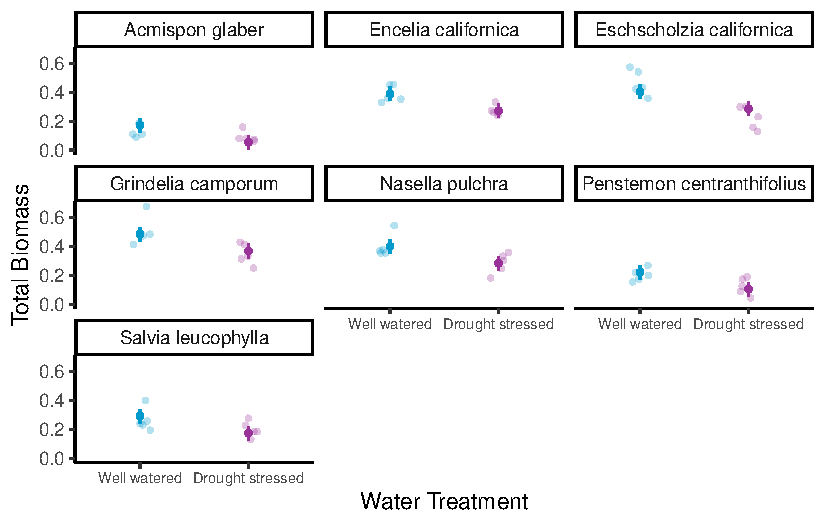
\includegraphics{ENVS193DS_Homework3_files/figure-pdf/unnamed-chunk-4-1.pdf}

\subsection{d.~Write a caption for your
visualization.}\label{d.-write-a-caption-for-your-visualization.}

Figure 1. Total Biomass of 7 native California plant species under
different water treatments. Each plot compares the total biomass of a
plant species when they are well watered versus drought stressed. Blue
indicates well watered and purple indicates drought stressed. Each plot
displays the average biomass and a 95\% confidence interval. Data
Source: Valliere J, Zhang J, Sharifi M, Rundel P (2019) \emph{Can we
condition native plants to increase drought tolerance and improve
restoration success?} https://doi.org/10.5061/dryad.v0861f7.

\subsection{e. Write a 3-4 sentence results
section.}\label{e.-write-a-3-4-sentence-results-section.}

Your answer should be in paragraph form and address the following
points:

what predictors ``best'' described total mass (include model statistics
here)? on average, what differences did you find between water
treatments? on average, what differences did you find between species?

\section{Problem 2. Affective
visualization}\label{problem-2.-affective-visualization}

\subsection{a. Describe in words what an affective visualization could
look like for your personal data (3-5
sentences)}\label{a.-describe-in-words-what-an-affective-visualization-could-look-like-for-your-personal-data-3-5-sentences}

Since my data is about crocheting, I want to make icons of the projects
that I've completed. I could do them in different sizes relative to the
time I spent on each with a border indicating pattern type and
difficulty, and highlighted according to type of yarn. I would like to
organize them chronologically and have an additional icon indicating the
day of the week and time of day I crochet the most.

\subsection{b. Create a sketch (on paper) of your
idea.}\label{b.-create-a-sketch-on-paper-of-your-idea.}

\begin{verbatim}
![Affective Visualization Sketch](images/affectivesketch.jpeg)
\end{verbatim}

\subsection{c.~Make a draft of your
visualization.}\label{c.-make-a-draft-of-your-visualization.}

\begin{verbatim}
![Crochet Data Affective Visualization](images/affectivecrochet.jpeg)

![Key](images/affectivekey.jpeg)
\end{verbatim}

\subsection{d.~Write an artist
statement.}\label{d.-write-an-artist-statement.}

I was very inspired by Stefanie Posavec and Giorgia Lupi's Dear Data
project and wanted to do a similar collage-type representation with
icons, shapes, colors, and borders representing my data. For my
visualization I used my iPad to create a drawing in Procreate with icons
for each project I completed this quarter. This visualization shows how
much time I spent on each project (size), what kind of yarn I used
(highlight color), pattern (border), and pattern level (shape).
Additionally I wanted to represent my crocheting habits throughout the
week so I added the days of the week, with size representing average
time spent per day and a sun icon indicating the time of day that I
tended to crochet. I drew it all by hand and tried to represent the
stitches and colors that I used for each project.

\section{Problem 3. Statistical
critique}\label{problem-3.-statistical-critique}

\subsection{a. Revisit and summarize}\label{a.-revisit-and-summarize}

The authors used 3 Kruskal Wallis Tests and one U Test to address their
main research question, is illegal fishing occurring in this Brazilian
MPA and if so, when? The Kruskal Wallis Tests analyze average fishing
vessel detections on three different temporal scales: by year, month,
and quarterly. Additionally, they performed a U test to add an
additional comparison of fishing vessel detections to lobster fishing
season.

\begin{figure}[H]

{\centering 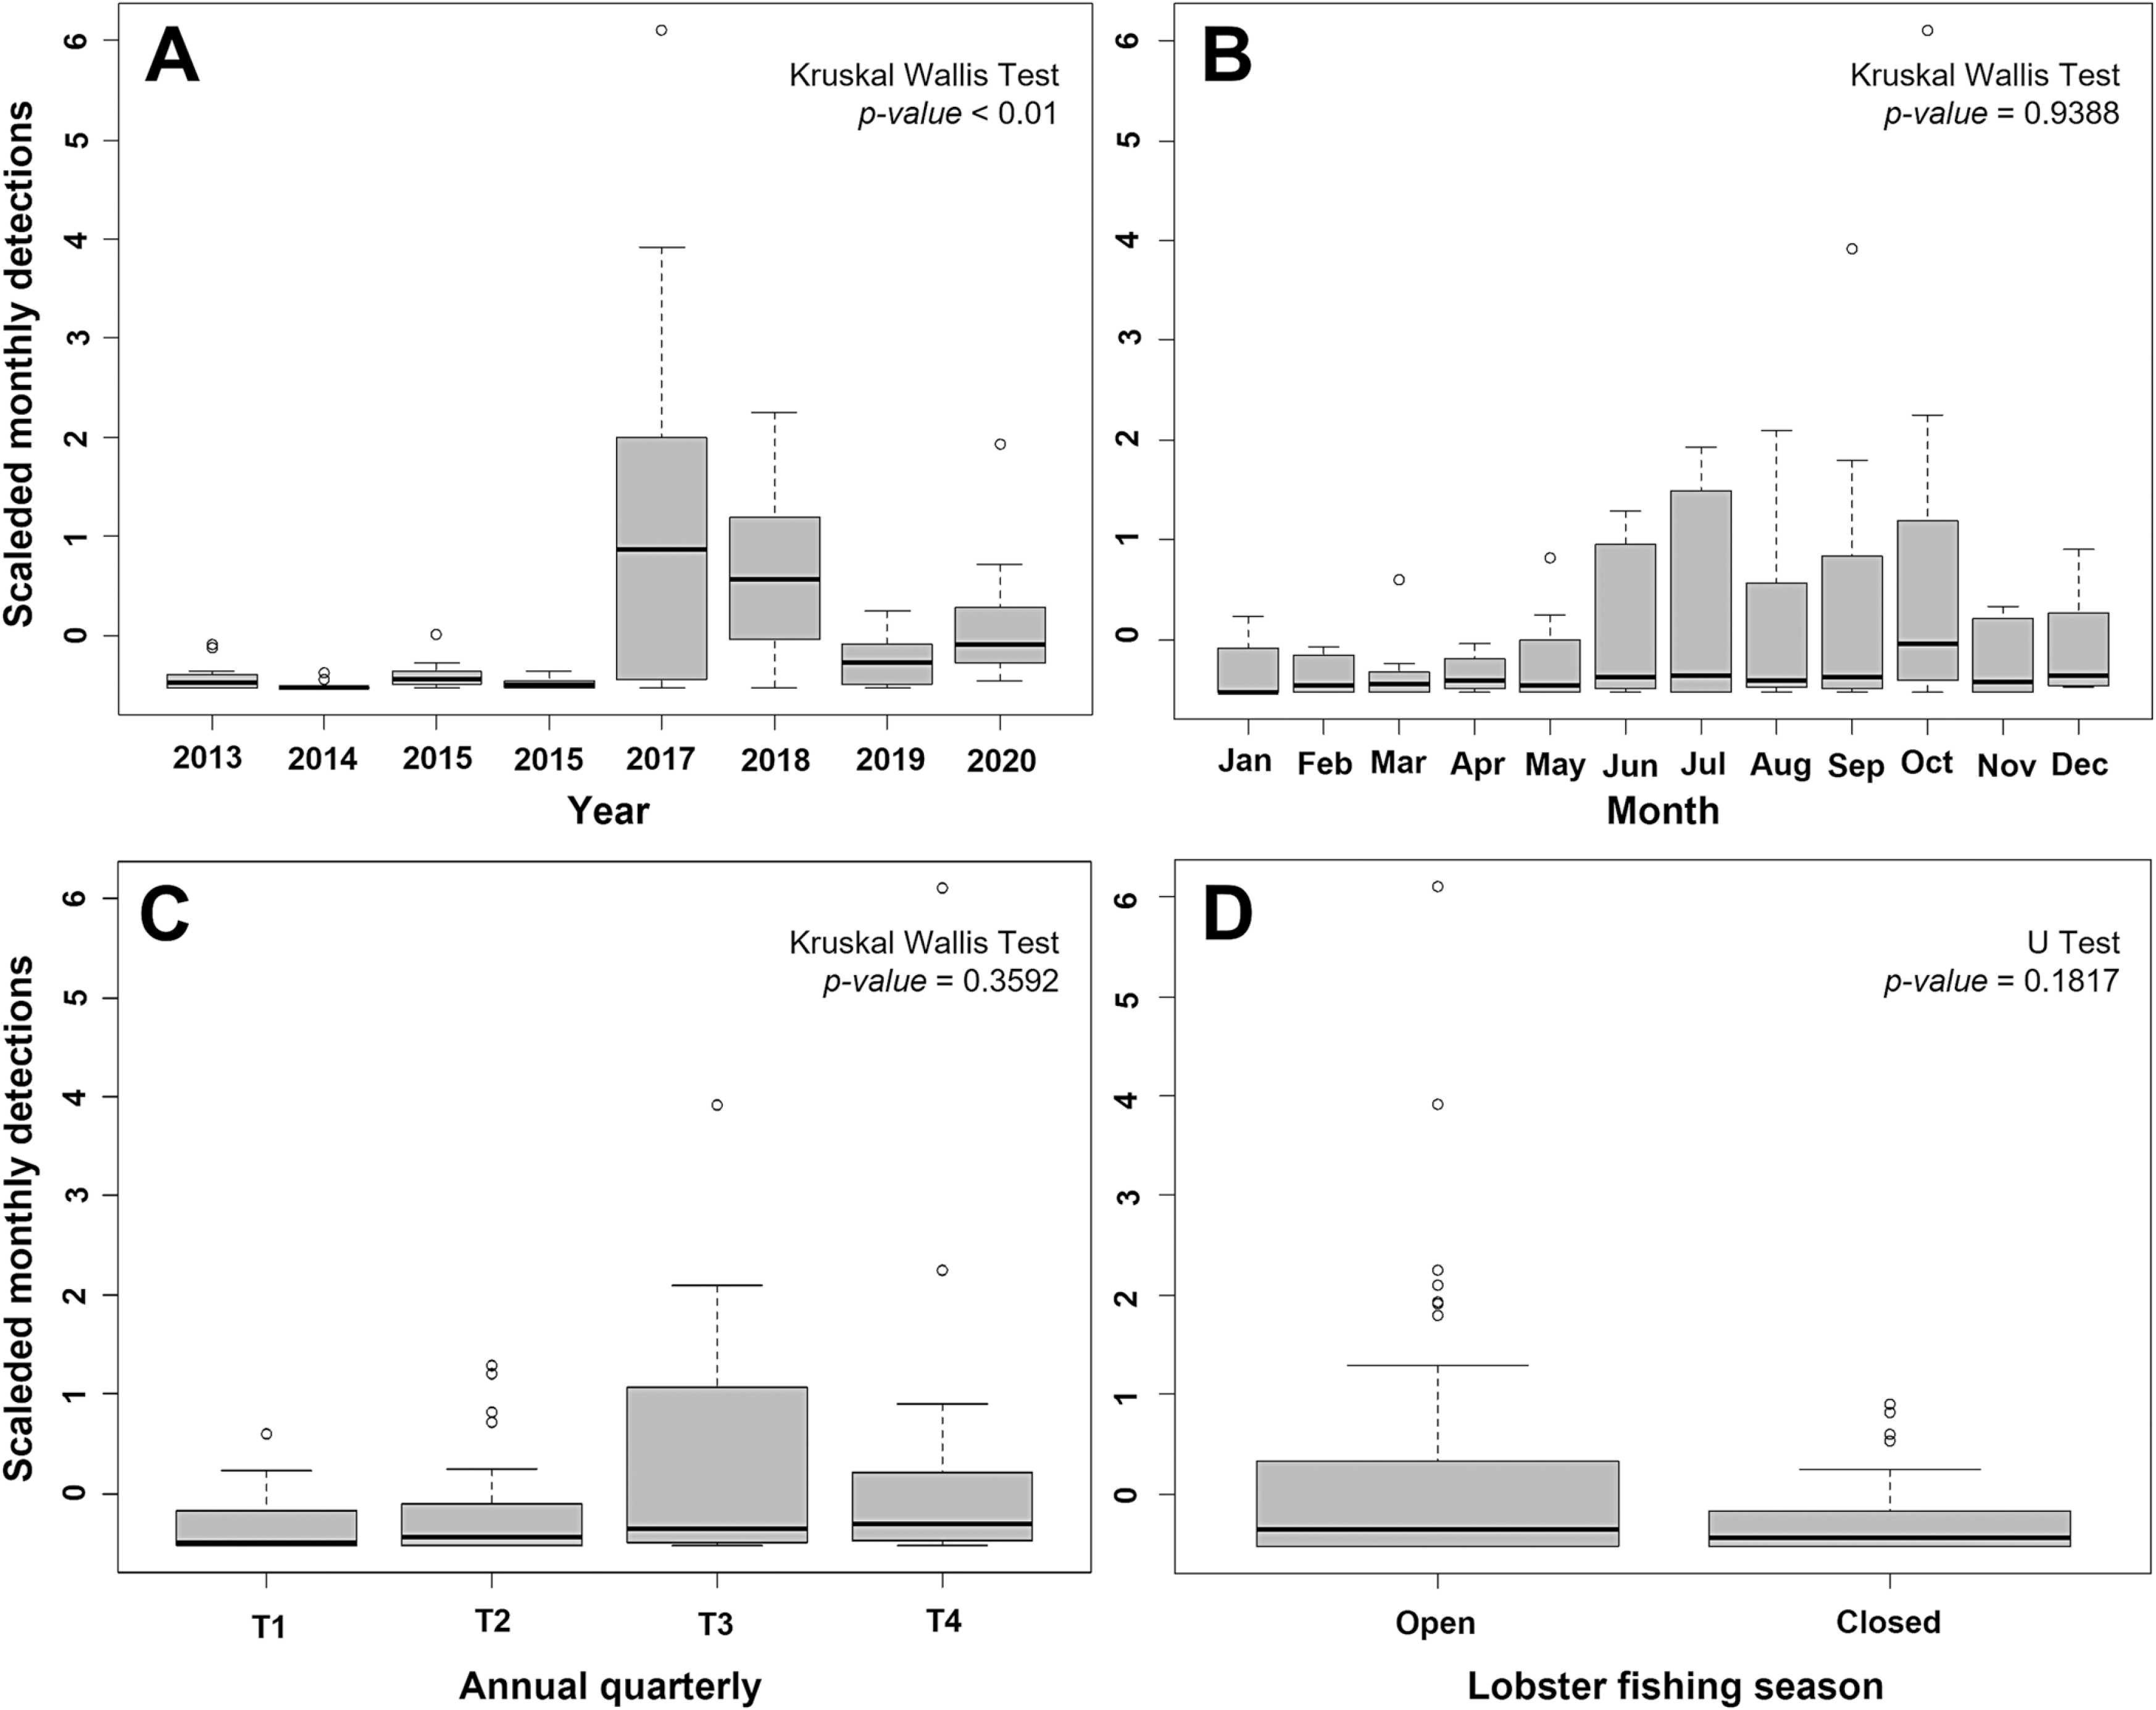
\includegraphics{images/193statcritic.jpg}

}

\caption{Table: Fishing vessel detections within APACC yearly, month,
quarterly, and according to lobster fishing season (2013-2020)}

\end{figure}%

\subsection{b. Visual clarity}\label{b.-visual-clarity}

The authors visually represented their data very clearly, everything is
appropriately titled and labeled. I think that the temporal scale on the
x axis and fishing detection on the y-axis is not only logical but very
easy to read an understand. The charts all communicate the same message
- the average fishing vessel detections and the different comparisons
they use are very clear in the charts. They represent the data using box
and whisker plots, so mean and standard error are included, although,
the underlying data isn't included but they did add in the outliers.

\subsection{c.~Aesthetic clarity}\label{c.-aesthetic-clarity}

There is little to no ``visual clutter'' in this visualization. I think
there is a high data:ink ratio because there are very few, if any,
aesthetic elements and all of the elements included are relevant data,
labels, or statistical tests.

\subsection{d.~Recommendations}\label{d.-recommendations}

I don't think there is anything that I would recommend taking out, if
anything, they could have added some color to make it more visually
engaging as it is quite a mundane representation. While it is clear that
the plots represent different temporal scales, a different color for
each chart would make this difference apparent at first glance. I think
adding the underlying data very transparently would provide a bit more
context particularly to the Lobster Fishing Season plot as there a quite
a few outliers. Since they list their p-value on the plot I think there
should be some indication of the significance level either as astrix on
the charts or in the caption.



\end{document}
